\chapter{El calendario de quemas: del registro a la interpretación}\label{cap:calendario}

\objetivos{\begin{itemize}
\item Construir un calendario sin confundir ausencia de detecciones con ausencia de observación.
\item Definir una referencia estacional y comparar el mismo periodo de distintos años.
\item Calcular anomalías, percentiles y fechas que describen la temporada de actividad.
\item Distinguir variabilidad histórica, incertidumbre de calibración y capacidad predictiva.
\item Leer un caso reproducible con detecciones reales de Perú.
\end{itemize}}

\FloatBarrier
\section{Una pregunta que sí puede responderse}

Un gestor pregunta: <<¿cuándo conviene reforzar la vigilancia?>>. Un archivo con miles de
coordenadas todavía no responde. Es necesario convertirlo en una descripción del tiempo:
cuándo suele concentrarse la actividad registrada, cuánto varía entre años y qué está
ocurriendo en comparación con una referencia. A esa descripción la llamaremos calendario.

La palabra \emph{quemas} requiere cuidado. Los datos de fuego activo no identifican por sí
solos la intención de quien inició el fuego. Un punto no permite decidir si fue una quema
agrícola autorizada, un incendio forestal o alguna otra fuente térmica. Filtrar fuentes
estáticas conocidas ayuda, pero no convierte el resto en un catálogo de incendios. El título
del producto puede ser <<calendario de actividad de fuego detectada>>; debajo debe aparecer
la unidad exacta. La estacionalidad de los registros de fuego activo tiene una larga historia
de estudio, pero cambia con el sensor y con la región.\fuente{giglio-season}

Este capítulo usa \textbf{datos reales de Perú}. Los números proceden de los archivos
nacionales anuales publicados por NASA FIRMS, conservados junto con el libro.\fuente{firms-country}
La física de los primeros capítulos explica su origen; la estadística y la armonización
explican qué transformaciones son defendibles. Aquí aprendemos a leer el resultado.

\FloatBarrier
\section{La ficha del caso peruano}\label{sec:peru-ficha}

Se descargaron los años completos de 2013 a 2024, doce archivos MODIS y doce VIIRS/Suomi NPP.
El archivo de procedencia registra para cada CSV su URL, fecha de descarga, número de filas,
versiones y huella SHA-256. No usamos un mapa copiado de otra aplicación: los conteos se
recalculan desde esas filas.

\begin{table}[ht]
\centering\renewcommand{\arraystretch}{1.2}
\begin{tabularx}{\textwidth}{l>{\raggedright\arraybackslash}X}
\toprule
Decisión & Configuración del caso \\
\midrule
Área & Perú, selección nacional distribuida por FIRMS \\
Periodo & Enero de 2013 a diciembre de 2024 \\
Plataformas & Aqua para MODIS; Suomi NPP para VIIRS, siempre separadas \\
Paso & Solo detecciones diurnas: \texttt{daynight=D} \\
Tipo & Solo filas con \texttt{type=0}; no prueba la causa del fuego \\
Confianza & MODIS: al menos 30; VIIRS: nominal o alta \\
Rejilla & $0{,}05^\circ$ por $0{,}05^\circ$, origen $(-90^\circ,-180^\circ)$ \\
Tiempo & Fecha local UTC$-$5; una clave por celda y día \\
Referencia del calendario & VIIRS/Suomi NPP, 2013--2023; 2024 se compara aparte \\
Cobertura & Sin corrección por nubes o por falta de pasadas \\
\bottomrule
\end{tabularx}
\caption{Contrato del análisis peruano. Cambiar un filtro cambia la población de datos y obliga
a recalcular la referencia. Los dos filtros de confianza son decisiones de selección, no
umbrales de probabilidad equivalentes.}
\label{tab:contrato-peru}
\end{table}

Entre ambos sensores los archivos contienen \PeruFilas{} filas; después de seleccionar
plataforma, día, tipo y confianza y quitar duplicados idénticos quedan \PeruAceptadas{}
detecciones. Todavía no son celdas-día: varias detecciones pueden compartir la misma clave.
En este conjunto diurno la conversión a UTC$-$5 conserva el año de cada archivo; el programa
lo comprueba. En un análisis nocturno habría que descargar también los días adyacentes al
periodo para no cortar una noche en la frontera del año.

\begin{atencion}[Una auditoría que cambia el análisis]
Los archivos MODIS descargados no tienen una etiqueta de versión uniforme: aparece
\texttt{6.2} en 2013--2017, \texttt{6.03} en 2018--2022 y \texttt{61.03} en 2023--2024.
No interpretamos el número decimal como una colección sin consultar su documentación ni
declaramos homogénea la serie entera. El calendario de este capítulo usa únicamente VIIRS,
cuya etiqueta es \texttt{2} en los doce archivos. La demostración de calibración del
capítulo~\ref{cap:aplicacion} se restringe a 2018--2022, con etiquetas constantes.
Para una serie MODIS larga de calidad científica hay que solicitar un archivo reprocesado
homogéneo y volver a validar. Encontrar esta limitación forma parte del trabajo.
\end{atencion}

\FloatBarrier
\section{Qué número ocupa cada casilla}

Sea $g$ una celda, $d$ un día y $s$ una plataforma. Definimos
\begin{equation}\label{eq:presencia}
 I_{s,g,d}=\begin{cases}
 1,&\text{si hay al menos una detección aceptada},\\
 0,&\text{si no hay detecciones en el registro disponible}.
 \end{cases}
\end{equation}
En esta definición, el cero describe el \emph{registro}. Para interpretarlo como un resultado
negativo de una observación válida hace falta información adicional de cobertura. La
actividad registrada de un área $R$ en el mes $m$ del año $y$ es
\begin{equation}\label{eq:actividad}
 C_{s,y,m}=\sum_{g\in R}\sum_{d\in(y,m)} I_{s,g,d}.
\end{equation}
Tiene unidades de celdas-día. Si una misma celda presenta detecciones durante tres días,
aporta tres unidades. Si veinte puntos caen en ella el mismo día, aporta una. Una región con
diez celdas puede aportar como máximo 310 celdas-día en un mes de 31 días. No son hectáreas ni
incendios independientes.

\begin{ejemplo}{sumar días y unir observaciones}
Supón tres celdas de Perú: el día 1 se detecta fuego en A y B; el día 2, en B; el día 3,
en A, B y C. ¿Qué actividad se registra? ¿Cuántas celdas distintas aparecen?
\solucion La suma diaria es $2+1+3=6$ celdas-día. Las celdas distintas son tres.
Si una pasada nocturna vuelve a ver B el día 1, el indicador diario total sigue valiendo
uno en B. Sumar las tablas diurna y nocturna daría una duplicación; hay que unir sus claves.
Si se desean dos indicadores por franja horaria, pueden mantenerse separados y nombrarse
explícitamente como celdas-día-franja.
\end{ejemplo}

Esta unidad está acotada. Si una conversión $rC$ supera el máximo de celdas-día posibles,
no es un conteo físico válido de presencia. Puede definirse como un \emph{índice de actividad
equivalente}, con sus propias unidades, o revisarse el modelo con una formulación acotada.
Redondearlo a un entero y llamarlo número de incendios ocultaría el problema.

\FloatBarrier
\section{Tres formas distintas de no ver un foco}

Imagina que el lunes el sensor observa una celda despejada y no detecta fuego; el martes
una nube oculta la celda; el miércoles falta el archivo de la pasada. Una tabla que solo
contiene detecciones positivas puede quedar vacía los tres días. Sin embargo, los tres
estados son diferentes.

\begin{figure}[ht]
\centering
\begin{tikzpicture}[node distance=7mm]
\node[caja,text width=4.1cm,minimum height=2.1cm,fill=bosqueClaro] (a) {\textbf{Observación válida}\\sin detección\\resultado negativo\\observado};
\node[caja,text width=4.1cm,minimum height=2.1cm,fill=cenizaClaro,right=of a] (b) {\textbf{Celda tapada}\\sin detección\\estado del suelo\\desconocido};
\node[caja,text width=4.1cm,minimum height=2.1cm,fill=fuegoClaro,right=of b] (c) {\textbf{Archivo ausente}\\sin registro\\fallo de disponibilidad};
\node[caja,below=10mm of b,text width=8cm] (d) {En el CSV de puntos, los tres pueden producir cero filas};
\draw[flujo] (a.south)--(d.north west);\draw[flujo] (b)--(d);\draw[flujo] (c.south)--(d.north east);
\end{tikzpicture}
\caption{Una ausencia en una tabla de detecciones no basta para reconstruir la oportunidad de
observación. Esquema conceptual; no representa tres fechas medidas.}
\label{fig:estados-cobertura}
\end{figure}

Si disponemos de una máscara de cobertura, podemos definir $O_{g,d}=1$ cuando se cumplió
un criterio explícito de observación válida. No basta que alguna parte de una celda grande
estuviera despejada: hay que fijar qué fracción, en qué pasada y con qué máscara. Entonces
\begin{equation}\label{eq:tasa-observada}
 f_m=\frac{\sum I_{g,d}O_{g,d}}{\sum O_{g,d}}
\end{equation}
describe la fracción de celdas-día observables que registraron al menos una detección.
Es una frecuencia \emph{condicionada a la observación}, no una corrección automática de la
actividad oculta por nubes. Si las condiciones nubosas están relacionadas con las quemas,
lo observado no es una muestra aleatoria del resto.

\begin{ejemplo}{el denominador importa}
En una región se registran 12 celdas-día con detección entre 300 celdas-día observables.
En otra se registran 8 entre 100. Compara los resultados.
\solucion Los conteos son 12 y 8, pero las frecuencias observadas son $12/300=0{,}04$ y
$8/100=0{,}08$. La segunda es el doble. No podemos calcular esos denominadores contando
filas del CSV de focos: necesitaríamos también las observaciones sin detección.
\end{ejemplo}

En el caso peruano de este libro no descargamos máscaras de observación. Por eso mostramos
actividad \emph{detectada sin ajuste de cobertura}. Los avisos de interrupciones de la
misión son otra fuente necesaria para investigar meses extraños.\fuente{outages}
Un archivo anual con datos no garantiza que todos sus días estén completos.

\FloatBarrier
\section{Leer el calendario de Perú}

La figura~\ref{fig:peru-calendario} coloca los meses en columnas y los años en filas.
Cada rectángulo contiene el resultado de la ecuación~\eqref{eq:actividad} para VIIRS/Suomi NPP.
La escala cromática es compartida: un color no cambia de significado al saltar a otra fila.

\begin{figure}[!htbp]
\centering
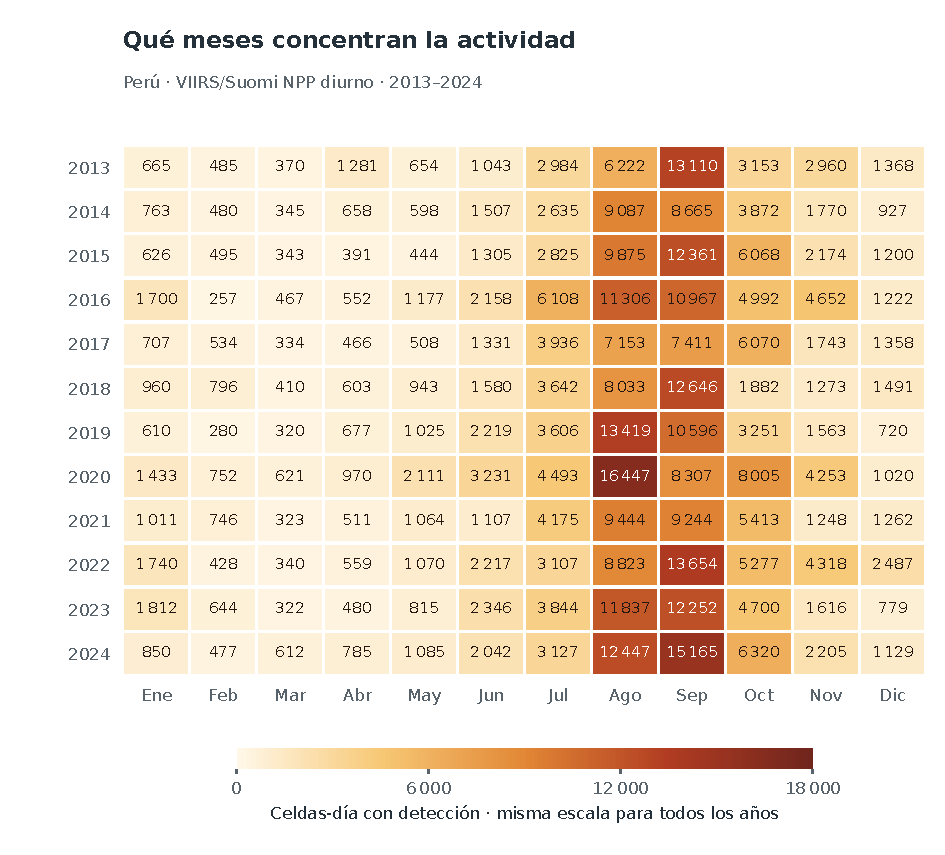
\includegraphics[width=\textwidth]{figuras/peru_calendario.pdf}
\caption{\textbf{Datos reales de Perú, 2013--2024.} Actividad diurna registrada por VIIRS/Suomi
NPP, tipo 0 y confianza nominal/alta, agrupada en celdas de $0{,}05^\circ$ y día local.
No se suman NOAA-20 ni NOAA-21. Fuente: CSV nacionales de NASA FIRMS; cálculo propio
reproducible en \texttt{scripts/analizar\_peru.py}. Sin corrección de cobertura ni nubes.}
\label{fig:peru-calendario}
\end{figure}

Primero se lee verticalmente: ¿el mismo mes tiende a ser activo en muchos años? Eso sugiere
un componente estacional. Luego se lee horizontalmente: ¿un año concentra su actividad en
pocos meses o la distribuye más? Finalmente se comparan filas: ¿hay un año distinto? Cada
pregunta es diferente. Un color intenso en septiembre no demuestra por sí solo una anomalía:
septiembre puede ser habitualmente intenso.

Hay un límite espacial importante. Perú contiene costa, sierra y selva, con climas y usos
del suelo distintos. Una curva nacional puede mezclar temporadas regionales diferentes.
Sirve para aprender el procedimiento y describir el conjunto; no debe convertirse en una
fecha única de preparación para cada municipio. Para Junín se necesitaría recortar las
detecciones con un límite administrativo documentado y repetir \emph{todo} el cálculo.
Un rectángulo alrededor de Huancayo no equivale al departamento de Junín.

\FloatBarrier
\section{Qué significa lo habitual}

\begin{definicion}{referencia estacional}
Una referencia estacional es la distribución histórica de una misma variable, en una misma
región y una misma posición del calendario, calculada con un periodo de referencia declarado.
Comparar un septiembre con otros septiembres controla la parte más evidente de la estacionalidad.
\end{definicion}

La referencia de este caso son los once años 2013--2023. Reservamos 2024 para compararlo.
Para cada mes calculamos la mediana y los percentiles 10 y 90 de sus once valores. Usamos
interpolación lineal: si los valores ordenados son $x_{(1)},\ldots,x_{(n)}$, la posición
del percentil $p$ es $h=1+(n-1)p$, con $p$ entre cero y uno. Se interpola entre las dos
posiciones vecinas. Con once años, $p=0{,}9$ da $h=10$: el percentil 90 es el décimo valor
ordenado. Explicitar la convención evita diferencias entre programas.

\begin{figure}[!htbp]
\centering
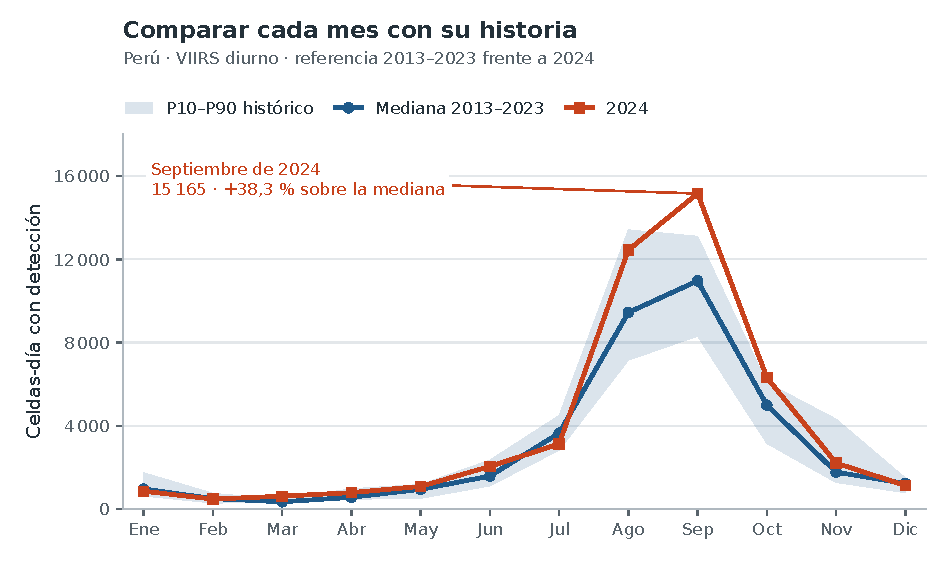
\includegraphics[width=\textwidth]{figuras/peru_perfil.pdf}
\caption{El mismo registro real de Perú, comparado por mes. La banda es variabilidad histórica
entre años; \textbf{no} es un intervalo de confianza de la mediana ni un pronóstico. Todos los
valores usan la selección de la tabla~\ref{tab:contrato-peru}.}
\label{fig:peru-perfil}
\end{figure}

Una referencia fija facilita comparar versiones de la aplicación: <<respecto de 2013--2023>>
siempre quiere decir lo mismo. Una referencia móvil se adapta a cambios recientes, pero
también cambia la vara de medir. Si cada año se actualiza, deben conservarse su versión y
los años que la integran. No existe una elección universalmente correcta; la elección
depende de si se quiere describir una anomalía respecto de un pasado fijo o del pasado reciente.

\begin{atencion}[Once años no son once certezas]
Los años pueden estar relacionados entre sí y el sistema de observación puede cambiar.
Una mediana robusta frente a un valor extremo no corrige esas dependencias ni elimina una
tendencia. Además, la serie nacional de once años no es una normal climatológica de treinta
años. En el libro la llamamos referencia histórica, indicando su duración.
\end{atencion}

\FloatBarrier
\section{Anomalía no significa automáticamente emergencia}

Si $b_m$ es la mediana de referencia y $C_m$ la actividad que comparamos, definimos
\begin{align}
 \Delta_m &= C_m-b_m,\label{eq:anom-absoluta}\\
 a_m &=100\left(\frac{C_m}{b_m}-1\right),\qquad b_m>0.\label{eq:anom-relativa}
\end{align}
La primera mide cuántas celdas-día adicionales aparecen en el registro; la segunda, la
diferencia relativa en porcentaje. Ambas tienen utilidad. Pasar de 1 a 4 produce una
anomalía del 300\,{}\%, pero una diferencia absoluta de solo tres unidades. Pasar de 4000 a
6000 produce un 50\,{}\% y dos mil unidades adicionales. El porcentaje por sí solo no
ordena la magnitud operativa del problema.

\begin{ejemplo}{septiembre de 2024 en Perú}
Con nuestra selección de datos, septiembre de 2024 contiene \PeruSeptActual{} celdas-día.
La mediana de septiembre de 2013--2023 es \PeruSeptMediana{} y su percentil 90 es
\PeruSeptQnoventa{}. ¿Cómo se expresa la diferencia?
\solucion Aplicando la ecuación~\eqref{eq:anom-relativa}, la diferencia respecto de la
mediana es \PeruSeptAnomalia{} por ciento. Esta cifra se refiere a actividad \emph{detectada}
por un sensor, con una rejilla y unos filtros concretos. No es el porcentaje de superficie
quemada ni el aumento del número de incendios reportados por las autoridades. Puede
reproducirse consultando la fila de septiembre en \texttt{datos/peru\_climatologia.csv}.
\end{ejemplo}

Si $b_m=0$, la razón no existe. No añadimos uno de forma silenciosa: cambiaría el significado
del indicador. Se puede informar <<hay detecciones; la mediana de referencia es cero>>,
mostrar la diferencia absoluta y ampliar la ventana temporal. Cuando el valor de referencia
es muy pequeño, incluso una razón definida es inestable. Un umbral mínimo para mostrar
porcentajes debe justificarse y mantenerse fijo.

Otra forma de describir una observación es su posición respecto de los años históricos.
Si supera a los once septiembres de referencia, es mayor que todos los valores de esa
muestra. No significa que su periodo de retorno sea infinito, ni que tenga probabilidad
uno de causar daños. Una muestra corta informa poco sobre los extremos.

\subsection{Desviación estándar y medidas robustas}

Con media $\bar C_m$ y desviación muestral $s_m$, el puntaje
\begin{equation}
 z_m=\frac{C_m-\bar C_m}{s_m}
\end{equation}
expresa cuántas desviaciones separan el valor de la media. Es una escala, no una prueba
automática de significación. Convertir $z=2$ en una probabilidad exige un modelo de
distribución que un conteo de fuegos asimétrico quizá no cumpla.

Una alternativa usa la mediana y la desviación absoluta mediana,
\begin{equation}
 \operatorname{MAD}=\operatorname{mediana}_y|C_{y,m}-b_m|,
 \qquad z_m^{\mathrm{rob}}=\frac{C_m-b_m}{1{,}4826\operatorname{MAD}}.
\end{equation}
El factor 1,4826 hace comparable la escala con una desviación estándar bajo normalidad;
no vuelve normales los datos. Si MAD es cero, el puntaje no se calcula. Para un público
general, mediana, rango histórico y diferencia absoluta suelen explicar más que una sigla.
La identificación de valores atípicos debe distinguir una señal interesante de un error
de medición o de un modelo inadecuado.\fuente{nist}

\FloatBarrier
\section{Cuándo empieza la temporada}

La pregunta tiene varias respuestas posibles. El primer foco del año depende mucho de
una detección aislada. El mes de máximo conteo es inestable si hay dos picos parecidos.
Una alternativa más gradual usa la fracción acumulada de actividad anual.

Para un año con actividad total positiva, definimos
\begin{equation}\label{eq:fraccion-estacional}
 p_{y,m}=\frac{C_{y,m}}{\sum_{j=1}^{12}C_{y,j}},\qquad
 \bar p_m=\frac{1}{n}\sum_y p_{y,m},\qquad
 F_m=\sum_{j=1}^{m}\bar p_j.
\end{equation}
Normalizar cada año antes de promediar da el mismo peso a todos los años válidos. En cambio,
dividir la suma de todos los agostos entre la suma de todos los años da más peso a los años
de gran actividad. Son preguntas distintas: una describe un año típico en forma, la otra
distribuye todas las unidades registradas durante el periodo.

\begin{figure}[!htbp]
\centering
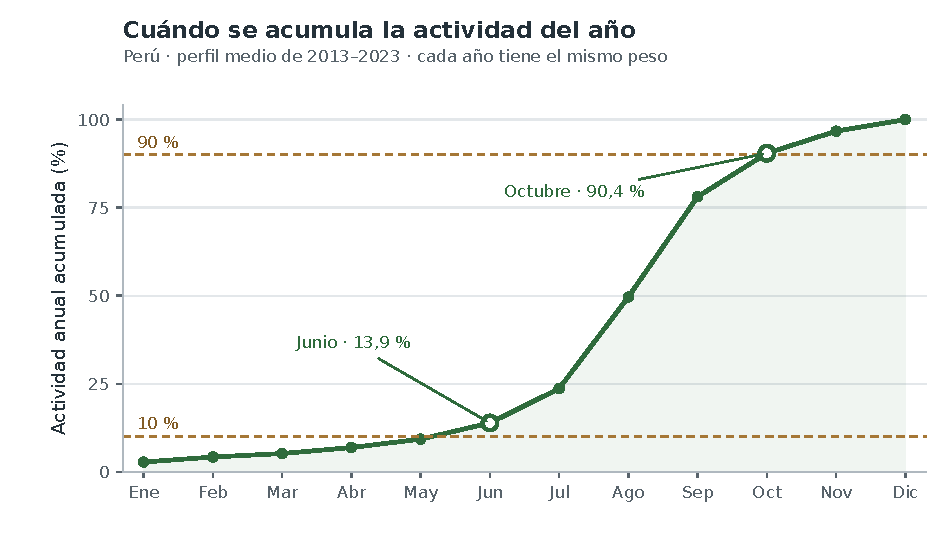
\includegraphics[width=\textwidth]{figuras/peru_acumulado.pdf}
\caption{Fracción acumulada media del año para Perú, VIIRS diurno, 2013--2023. Cada año se
normaliza por su propio total antes del promedio. Las líneas del 10 y el 90\,{}\% ilustran
una definición de ventana central de actividad, no umbrales oficiales de alerta.}
\label{fig:peru-acumulado}
\end{figure}

Podemos llamar comienzo de la ventana central al primer mes que alcanza el 10\,{}\% y
final al que alcanza el 90\,{}\%. Esa ventana contiene aproximadamente el 80\,{}\% central
de la actividad de la distribución estacional. Con datos mensuales la resolución es mensual:
dar un día exacto mediante interpolación supondría que la actividad se reparte uniformemente
dentro del mes. Si se necesita una fecha, se repite el cálculo con días o semanas y se
explica el suavizado.

\begin{ejemplo}{una cifra estacional reproducible}
En el perfil peruano de 2013--2023, la suma de las fracciones medias de agosto, septiembre
y octubre es \PeruASO{} por ciento. ¿Significa que cada año tuvo exactamente esa fracción?
\solucion No. Se normalizó cada año y se promediaron sus fracciones. Un año puede anticipar
o retrasar la temporada. La cifra resume la concentración media de la actividad detectada
en esos tres meses; su variabilidad se estudia conservando las fracciones de cada año.
\end{ejemplo}

En una zona con dos temporadas separadas, una sola ventana 10--90 puede incluir un periodo
intermedio poco activo. En una zona cuya temporada cruza diciembre hay que elegir un año
de actividad, por ejemplo julio a junio, y conservarlo. El calendario debe seguir al
fenómeno, no imponerle por comodidad la forma del año civil.

\FloatBarrier
\section{Meses incompletos y suavizado}

El 12 de septiembre todavía no existe el total de septiembre. Comparar sus primeros doce
días con meses completos produce una falsa caída. Hay dos comparaciones honestas: esperar
a cerrar el mes o comparar del 1 al 12 con del 1 al 12 de cada año histórico. En el segundo
caso deben utilizarse también archivos con una madurez semejante, o marcar que lo reciente
es provisional y puede revisarse.

Multiplicar un conteo parcial por $30/12$ es una proyección que supone un ritmo uniforme.
Puede servir como escenario simple, pero falla si la temporada está creciendo o si faltó
una pasada decisiva. No se etiqueta como total observado.

Para visualizar una serie diaria se puede suavizar con una media móvil. Una media centrada
de siete días en $d$ usa desde $d-3$ hasta $d+3$; una media retrospectiva usa desde $d-6$
hasta $d$. La centrada es útil para una figura histórica, pero conoce tres días del futuro.
No debe utilizarse sin cambios para evaluar una señal emitida en el día $d$.
Los métodos de evaluación temporal hacen explícita esta frontera entre pasado disponible
y futuro reservado.\fuente{forecast}

\FloatBarrier
\section{Qué incertidumbre dibujar}

Hay al menos tres bandas diferentes que podrían rodear una curva. La banda P10--P90 de la
figura~\ref{fig:peru-perfil} describe cómo variaron años pasados. Un intervalo de confianza
de la mediana describe la incertidumbre de estimar esa mediana con pocos años. Un intervalo
de predicción intenta cubrir una observación futura. Las tres bandas responden preguntas
distintas y no deben compartir una leyenda genérica de <<error>>.

En una serie armonizada aparece otra incertidumbre: la de la calibración. Si muchas
celdas usan la misma razón $r$, sus errores de conversión están relacionados. No se debe
sortear una razón independiente para cada celda: al sumar miles de celdas, esa simulación
haría desaparecer artificialmente la incertidumbre común.

Un procedimiento más fiel remuestrea bloques de años del periodo de ajuste, vuelve a
estimar una razón por estrato y aplica esa misma razón a todas las celdas del estrato en
cada réplica. Después construye el calendario de esa réplica. La dispersión final transmite
la incertidumbre estimada del ajuste. Sigue sin reconstruir fuegos ocultos ni corregir
sesgos desconocidos; su alcance debe escribirse junto a la banda.

\FloatBarrier
\section{De la anomalía a una decisión}

Una aplicación puede señalar <<actividad registrada por encima del P90 histórico>> y
proponer revisar las observaciones. Para llamarlo alerta predictiva tendría que demostrar
que una señal emitida con información disponible hasta hoy anticipa un resultado futuro
definido. Harían falta una ventana de anticipación, una variable objetivo, datos de
verificación y evaluación fuera de muestra. El calendario histórico es una pieza útil
para prepararse; por sí solo no predice dónde arderá mañana.

Además, al revisar muchos lugares aparecen valores extremos por casualidad. Si cincuenta
series independientes tienen cada una una probabilidad de 0,1 de superar cierto umbral
en un periodo, se esperan cinco superaciones, y la probabilidad de al menos una es
$1-0{,}9^{50}\approx99{,}5\,{}\%$. En la realidad hay dependencia espacial y umbrales
estimados, de modo que ese cálculo es solo una ilustración. Enseña por qué <<algo salió
rojo en el mapa>> no demuestra una emergencia.\fuente{isl}

Para evaluar señales operativas se necesita revisar persistencia, magnitud absoluta,
calidad de observación y un resultado independiente de los mismos datos usados para
crear la señal. Un percentil es un descriptor; una decisión también incorpora consecuencias
y conocimiento del territorio.

\resumen
\begin{itemize}
\item Una casilla puede contar detecciones, celdas-día o un índice equivalente. La unidad
debe conservarse desde el archivo hasta la pantalla.
\item Cero detecciones, celda no observable y archivo ausente son estados distintos.
\item La referencia compara el mismo mes, región, selección y unidad; se declara su periodo.
\item Una anomalía se acompaña de magnitud absoluta, referencia e información de cobertura.
\item El calendario real de Perú se reproduce desde los CSV de FIRMS y no constituye un
censo de incendios ni una estimación de área quemada.
\item Una temporada definida mediante acumulados es retrospectiva; no anticipa por sí sola
los incendios del año siguiente.
\end{itemize}

\ejercicios
\begin{enumerate}
\item A partir de \path{datos/peru_mensual.csv}, comprueba el total anual de VIIRS de 2024 por
dos caminos: sumando meses y contando las claves de celda-día del archivo original.
\item En una cuadrícula de 40 celdas, ¿cuál es el máximo de celdas-día de febrero de 2024?
¿Qué interpretación tendría una conversión que superara ese máximo?
\item Calcula para agosto la anomalía de 2024 respecto de la mediana 2013--2023 y contrástala
con la cifra \PeruAgostoAnomalia{} por ciento. Explica el efecto de usar una media.
\item Ordena los once septiembres de referencia y comprueba su percentil 90 con la convención
del texto. ¿Cuánto cambia si se excluye un solo año extremo?
\item Repite el perfil estacional dando a cada celda-día el mismo peso en todo el periodo,
en vez de dar el mismo peso a cada año. Explica por qué las curvas no tienen que coincidir.
\item Una API devuelve cero filas para un día. Enumera tres explicaciones distintas y qué
metadatos permitirían distinguirlas.
\item Diseña la comparación que mostrarías el 12 de septiembre. Indica exactamente qué
fechas usarías en cada año de referencia y qué dato futuro queda excluido.
\item Una mediana es cero y el valor actual es cinco. Redacta una frase informativa sin
inventar un porcentaje ni llamarlo incendio confirmado.
\item Describe cómo remuestrearías la incertidumbre de un calendario cuyas 2000 celdas
comparten una sola razón de calibración. ¿Por qué no sortear 2000 razones independientes?
\item Propón un criterio comprobable para afirmar que una herramienta anticipa actividad
con una semana de antelación. Separa variable objetivo, datos disponibles y periodo de prueba.
\end{enumerate}

\lecturas
La investigación de Giglio, Csiszar y Justice sobre distribución y estacionalidad del fuego
activo sitúa el calendario en su contexto científico.\fuente{giglio-season} Para evaluar
series sin introducir información futura, consulta el capítulo sobre herramientas de
pronóstico de Hyndman y Athanasopoulos.\fuente{forecast} El archivo de FIRMS y el programa
del caso peruano permiten practicar cada paso con datos reales, en lugar de memorizar
una curva estacional.\fuente{firms-country}
